
\documentclass[10pt,journal,compsoc]{IEEEtran}

% *** CITATION PACKAGES ***
%
\ifCLASSOPTIONcompsoc
  % IEEE Computer Society needs nocompress option
  % requires cite.sty v4.0 or later (November 2003)
  \usepackage[nocompress]{cite}
\else
  % normal IEEE
  \usepackage{cite}
\fi

\usepackage{mathptmx}
\usepackage{graphicx}
\usepackage{times}
%\usepackage{tabularx}
\usepackage{amsmath}
%\usepackage{url}
\usepackage{caption,subcaption}
\usepackage{multirow}
\usepackage{paralist}
\usepackage{listings}

\usepackage{color}
\definecolor{RED}{rgb}{1,0,0}
\definecolor{BLUE}{rgb}{0,0,1}
\newcommand{\FIXME}[1]{\textbf{\color{BLUE}{FIXME: #1}}}
\newcommand{\sref}[1]{Section~\ref{#1}}
\newcommand{\fig}[1]{Figure~\ref{#1}}

% suppress  single floating lines on top (widow) and bottom (club)
%  10000 is infinity
%  tradeoff: possible underful vboxes
\clubpenalty=10000
\widowpenalty=10000

% correct bad hyphenation here
\hyphenation{op-tical net-works semi-conduc-tor}


\begin{document}
%
% paper title
% Titles are generally capitalized except for words such as a, an, and, as,
% at, but, by, for, in, nor, of, on, or, the, to and up, which are usually
% not capitalized unless they are the first or last word of the title.
% Linebreaks \\ can be used within to get better formatting as desired.
% Do not put math or special symbols in the title.
\title{Equalizer 2.0\\Convergence of a Parallel Rendering Framework}
%
%
% author names and IEEE memberships
% note positions of commas and nonbreaking spaces ( ~ ) LaTeX will not break
% a structure at a ~ so this keeps an author's name from being broken across
% two lines.
% use \thanks{} to gain access to the first footnote area
% a separate \thanks must be used for each paragraph as LaTeX2e's \thanks
% was not built to handle multiple paragraphs
%
%
%\IEEEcompsocitemizethanks is a special \thanks that produces the bulleted
% lists the Computer Society journals use for "first footnote" author
% affiliations. Use \IEEEcompsocthanksitem which works much like \item
% for each affiliation group. When not in compsoc mode,
% \IEEEcompsocitemizethanks becomes like \thanks and
% \IEEEcompsocthanksitem becomes a line break with idention. This
% facilitates dual compilation, although admittedly the differences in the
% desired content of \author between the different types of papers makes a
% one-size-fits-all approach a daunting prospect. For instance, compsoc
% journal papers have the author affiliations above the "Manuscript
% received ..."  text while in non-compsoc journals this is reversed. Sigh.

%% Author and Affiliation (multiple authors with multiple affiliations)
\author{Stefan Eilemann\thanks{email: eilemann@gmail.com} \\ %
\and Renato Pajarola\thanks{email: pajarola@acm.org}}


\author{Stefan~Eilemann, David~Steiner and Renato Pajarola% <-this % stops a space
\IEEEcompsocitemizethanks{\IEEEcompsocthanksitem All authors are with the Visualization and MultiMedia Lab, Department of Informatics, University of Z\"urich.
\IEEEcompsocthanksitem S. Eilemann is also with the Blue Brain Project, Ecole
Polytechnique Federale de Lausanne.}}

% note the % following the last \IEEEmembership and also \thanks -
% these prevent an unwanted space from occurring between the last author name
% and the end of the author line. i.e., if you had this:
%
% \author{....lastname \thanks{...} \thanks{...} }
%                     ^------------^------------^----Do not want these spaces!
%
% a space would be appended to the last name and could cause every name on that
% line to be shifted left slightly. This is one of those "LaTeX things". For
% instance, "\textbf{A} \textbf{B}" will typeset as "A B" not "AB". To get
% "AB" then you have to do: "\textbf{A}\textbf{B}"
% \thanks is no different in this regard, so shield the last } of each \thanks
% that ends a line with a % and do not let a space in before the next \thanks.
% Spaces after \IEEEmembership other than the last one are OK (and needed) as
% you are supposed to have spaces between the names. For what it is worth,
% this is a minor point as most people would not even notice if the said evil
% space somehow managed to creep in.


% The paper headers
\markboth{Journal of \LaTeX\ Class Files,~Vol.~14, No.~8, August~2015}%
{Shell \MakeLowercase{\textit{et al.}}: Bare Demo of IEEEtran.cls for Computer Society Journals}
% The only time the second header will appear is for the odd numbered pages
% after the title page when using the twoside option.
%
% *** Note that you probably will NOT want to include the author's ***
% *** name in the headers of peer review papers.                   ***
% You can use \ifCLASSOPTIONpeerreview for conditional compilation here if
% you desire.



% The publisher's ID mark at the bottom of the page is less important with
% Computer Society journal papers as those publications place the marks
% outside of the main text columns and, therefore, unlike regular IEEE
% journals, the available text space is not reduced by their presence.
% If you want to put a publisher's ID mark on the page you can do it like
% this:
%\IEEEpubid{0000--0000/00\$00.00~\copyright~2015 IEEE}
% or like this to get the Computer Society new two part style.
%\IEEEpubid{\makebox[\columnwidth]{\hfill 0000--0000/00/\$00.00~\copyright~2015 IEEE}%
%\hspace{\columnsep}\makebox[\columnwidth]{Published by the IEEE Computer Society\hfill}}
% Remember, if you use this you must call \IEEEpubidadjcol in the second
% column for its text to clear the IEEEpubid mark (Computer Society jorunal
% papers don't need this extra clearance.)



% use for special paper notices
%\IEEEspecialpapernotice{(Invited Paper)}

% for Computer Society papers, we must declare the abstract and index terms
% PRIOR to the title within the \IEEEtitleabstractindextext IEEEtran
% command as these need to go into the title area created by \maketitle.
% As a general rule, do not put math, special symbols or citations
% in the abstract or keywords.
\IEEEtitleabstractindextext{%
  \begin{abstract}
    Developing complex, real world applications which utilize multiple GPUs and
    computers for 3D interactive rendering tasks can be a daunting task, in
    particular since it requires expertise in distributed systems and parallel
    rendering in addition to the application domain. We present a mature
    parallel rendering framework which provides a large set of features,
    algorithms and system integration for a wide range of real-world research
    and industry applications. Based on the basic architecture and
    implementation of the Equalizer parallel rendering framework presented in
    \cite{EMP:09}, we show how the generic algorithms are integrated in the
    framework to help application development in many different domains.
  \end{abstract}

  % Note that keywords are not normally used for peerreview papers.
  \begin{IEEEkeywords}
    Parallel Rendering, Scalable Visualization, Cluster Graphics, Immersive Environments, Display Walls
  \end{IEEEkeywords}
}


% make the title area
\maketitle


% To allow for easy dual compilation without having to reenter the
% abstract/keywords data, the \IEEEtitleabstractindextext text will
% not be used in maketitle, but will appear (i.e., to be "transported")
% here as \IEEEdisplaynontitleabstractindextext when the compsoc
% or transmag modes are not selected <OR> if conference mode is selected
% - because all conference papers position the abstract like regular
% papers do.
\IEEEdisplaynontitleabstractindextext
% \IEEEdisplaynontitleabstractindextext has no effect when using
% compsoc or transmag under a non-conference mode.



% For peer review papers, you can put extra information on the cover
% page as needed:
% \ifCLASSOPTIONpeerreview
% \begin{center} \bfseries EDICS Category: 3-BBND \end{center}
% \fi
%
% For peerreview papers, this IEEEtran command inserts a page break and
% creates the second title. It will be ignored for other modes.
\IEEEpeerreviewmaketitle

%----------------------------------------------------------------------
\begin{figure*}[ht]\center
  \includegraphics[width=2\columnwidth]{images/teaser} \\
  (a) \hfil \hfil (b) \hfil \hfil (c)
  \vspace{-2mm}
  \caption{Example Equalizer application use cases: (a) 192 Megapixel CAVE at
    KAUST running RTNeuron, (b) Immersive HMD with external tracked and
    untracked views running RTT DeltaGen for virtual car usability studies (c)
    Cave2 running a molecular visualization build using Omegalib.}
  \label{FIG_teaser}
\end{figure*}

%----------------------------------------------------------------------
% Computer Society journal (but not conference!) papers do something unusual
% with the very first section heading (almost always called "Introduction").
% They place it ABOVE the main text! IEEEtran.cls does not automatically do
% this for you, but you can achieve this effect with the provided
% \IEEEraisesectionheading{} command. Note the need to keep any \label that
% is to refer to the section immediately after \section in the above as
% \IEEEraisesectionheading puts \section within a raised box.
\IEEEraisesectionheading{\section{Introduction}\label{sec:introduction}}
%----------------------------------------------------------------------


Highlight integration of many features into a general framework vs one-off
research implemenation of one algorithm.


%----------------------------------------------------------------------
\section{Related Work}\label{sec:related}
%----------------------------------------------------------------------

In~\cite{EMP:09}, we presented the Equalizer parallel rendering framework. This
paper summarized the work in parallel rendering up to 2009. In the following we
will present the related work published since then. An extensive Programming and
User Guide provides in-depth documentation on using and programming
Equalizer~\cite{Eilemann:13}.

The concept of transparent OpenGL interception popularized by WireGL and
Chromium~\cite{HHNFAKK:02} has received little attention since 2009. While some
commercial implementations such as TechViz and MechDyne Conduit continue to
exist, on the research side only ClusterGL~\cite{NHM:11} has been
presented. ClusterGL employs the same approach as Chromium, but delivers a
significantly faster implementation of transparent OpenGL interception and
distribution for parallel rendering. CGLX~\cite{DK:11} tries to bring parallel
execution transparently to OpenGL applications, by emulating the GLUT API and
intercepting certain OpenGL calls. This approach works transparently for trivial
applications, but quickly requires the application developer to address the
complexities of a distributed application when mutable application state needs
to be synchronized across processes.

On the other hand, software for driving and interacting with tiled display walls
has received significant attention. Sage~\cite{Sage} and Sage2~\cite{Sage2} have
received significant attention. Sage is build entirely around the concept of a
shared framebuffer where all content windows are separate applications using
pixel streaming. It is no longer actively supported. Sage 2 is a complete,
browser-centric reimplementation where each application is a web application
distributed across browser instances. DisplayCluster~\cite{DC}, and its
continuation Tide, also implement the shared framebuffer concept of Sage, but
provide a few native content applications integrated into the display servers.

Equalizer itself has received significant attention to research and validate
parallel rendering performance, by using compression and region of interest
during compositing~\cite{MEP:10}, load-balancing resources for multi-display
installations~\cite{EEP:11}, asynchronous compositing and NUMA
optimizations~\cite{EBAHMP:12} as well as work queueing~\cite{SPEP:16}.

Various applications and frameworks have used Equalizer for new research in
visualization, such as the RTNeuron~\cite{HBBES:13}, an OpenGL renderer for
visualizing simulations of neucortical brain regions, Omegalib~\cite{Omegalib},
extending Equalizer for the hybrid 2D/3D environments such as the CAVE2,
visualization for remote sensing date~\cite{LK:09}, .

\cite{CKP:12} tiled display wall virtual environment


%------------------------------------------------------------------------------
\section{Performance}
%------------------------------------------------------------------------------

This section introduces new decomposition modes, runtime adaptations and other
optimizations to increase the rendering performance for a wide variety of
algorithms.

\subsection{New Decomposition Modes}

The initial version of Equalizer implemented sort-first (2D), sort-last (DB),
stereo (EYE) and multilevel decompositions \cite{EMP:09}. In the following we
present new decomposition modes and motivate their use case. \fig{fig:compounds}
provides an overview of the new modes. We describe their configuration in
same \textit{compound} framework introduced in \cite{EMP:09}

\begin{figure*}[ht]\center
  \begin{subfigure}[b]{0.24\textwidth}
    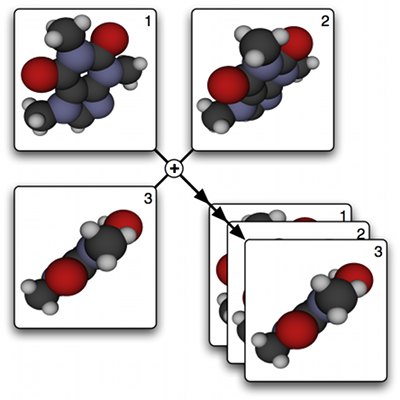
\includegraphics[width=\textwidth]{images/dplex}
  \end{subfigure}
  \begin{subfigure}[b]{0.24\textwidth}
    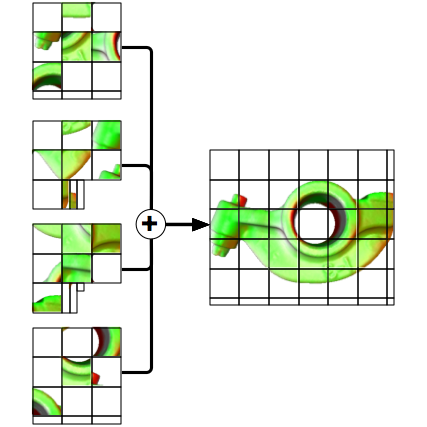
\includegraphics[width=\textwidth]{images/tile}
  \end{subfigure}
  \begin{subfigure}[b]{0.24\textwidth}
    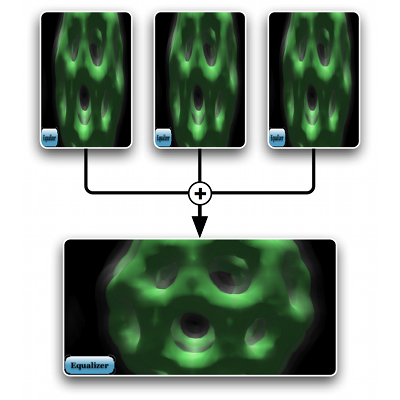
\includegraphics[width=\textwidth]{images/pixel}
  \end{subfigure}
  \begin{subfigure}[b]{0.24\textwidth}
    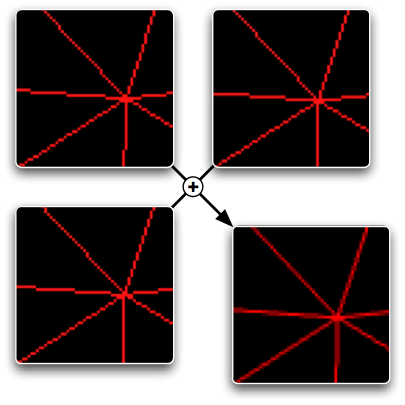
\includegraphics[width=\textwidth]{images/subpixel}
  \end{subfigure}\\[\medskipamount]
  \begin{subfigure}[t]{0.24\textwidth}
    {\tiny\begin{lstlisting}
compound {
  channel "destination"
  framerate_equalizer {}
  compound {
    channel "source1"
    phase 0 period 3
    outputframe  { name "frame" }
  }
  compound {
    channel "source2"
    phase 1 period 3
    outputframe  { name "frame" }
  }
  compound {
    channel "source3"
    phase 2 period 3
    outputframe  { name "frame" }
  }
  inputframe { name "frame" }
}
    \end{lstlisting}\vspace{24ex}}
    \caption{\label{fig:dplex}Time-Multiplex}
  \end{subfigure}
  \begin{subfigure}[t]{0.24\textwidth}
    {\tiny\begin{lstlisting}
compound {
  channel "destination"
  outputtiles {
    name "queue"
    size [ 64 64 ]
  }
  compound {
    channel "destination"
    inputtiles { name "queue" }
  }
  compound {
    channel "source1"
    inputtiles { name "queue" }
    outputframe {}
  }
  compound {
    channel "source2"
    inputtiles { name "queue" }
    outputframe {}
  }
  compound {
    channel "source3"
    inputtiles { name "queue" }
    outputframe {}
  }
  inputframe { name "frame.source1" }
  inputframe { name "frame.source2" }
  inputframe { name "frame.source3" }
}
    \end{lstlisting}}
    \caption{\label{fig:tiles}Tiles}
  \end{subfigure}
  \begin{subfigure}[t]{0.24\textwidth}
    {\tiny\begin{lstlisting}
compound {
  channel "dest"
  compound {
    channel "dest"
    pixel [ 0 0 3 1 ]
    outputframe { type texture }
  }
  compound {
    channel "source1"
    pixel [ 1 0 3 1 ]
    outputframe {}
  }
  compound {
    channel "source2"
    pixel [ 2 0 3 1 ]
    outputframe {}
  }
  inputframe { name "frame.dest" }
  inputframe { name "frame.source1" }
  inputframe { name "frame.source2" }
}
    \end{lstlisting}\vspace{21ex}}
    \caption{\label{fig:pixel}Pixel}
  \end{subfigure}
  \begin{subfigure}[t]{0.24\textwidth}
    {\tiny\begin{lstlisting}
compound {
  channel "dest"
  compound {
    channel "dest"
    subpixel [ 0 3 ]
    outputframe { type texture }
  }
  compound {
    channel "source1"
    subpixel [ 1 3 ]
    outputframe {}
  }
  compound {
    channel "source2"
    subpixel [ 1 3 ]
    outputframe {}
  }
  inputframe { name "frame.dest" }
  inputframe { name "frame.source1" }
  inputframe { name "frame.source2" }
}
    \end{lstlisting}\vspace{21ex}}
    \caption{\label{fig:subpixel}Subpixel}
  \end{subfigure}
  \caption{New Equalizer task decompositions and their compounds for parallel
    rendering}
  \label{fig:compounds}
\end{figure*}


\subsubsection{Time-Multiplex}

Time-multiplexing (\fig{fig:dplex}), also called AFR or DPlex, was first
implemented in \cite{BRE:05} for shared memory machines. It is however a better
fit for distributed memory systems, since the separate memory space makes
concurrent rendering of different frames easier to implement. While it increases
the framerate linearly, it does not decrease the latency between user input and
the corresponding output. Consequently, this decomposition mode is mostly useful
for non-interactive movie generation. It is transparent to Equalizer
applications, but does require the configuration latency to be equal or greater
than the number of source channels. Furthermore, to work in a multi-threaded,
multi-GPU configuration, the application needs to support running the rendering
threads asynchronously, as outlined in \sref{sec:threading}. The output frame
rate of the destination channel is smoothened using a frame rate equalizer
(\sref{sec:framerateEq}).

\subsubsection{Tiles and Chunks}\label{sec:tile}

Tile (\fig{fig:tiles}) and chunk decompositions are a variant of sort-first and
sort-last rendering, respectively. They decompose the scene into a predefined
set of fixed-size image tiles or database ranges. These tasks are queued and
processed by all source channels by polling a server-central queue. Prefetching
ensures that the task communication overlaps with rendering. As shown in
\cite{SPEP:16}, these modes provide better performance due to being inherently
load-balanced, as long as there is an insignificant overhead for the render task
setup. This mode is transparent to Equalizer applications.


\subsubsection{Pixel}

Pixel compounds (\fig{fig:pixel}) decompose the destination channel by
interleaving rows or columns in image space. They are a variant of sort-first
decomposition which works well for fill-limited applications which are not
geometry bound. Source channels cannot reduce geometry load through view frustum
culling, since each source channel has almost the same frustum (only shifted by
some pixels), but applied to a reduced 2D viewport. However, the fragment load
on all source channels is very similar due to the interleaved distribution of
pixels. This functionality is transparent to Equalizer applications, and the
default compositing implementation uses the OpenGL stencil buffer to blit pixels
onto the destination channel.

\subsubsection{Subpixel}

Subpixel compounds (\fig{fig:subpixel}) are similar to pixel compounds, but they
decompose the work for a single pixel, for example when using multisampling or
depth of field. Composition typically uses accumulation and averaging of all
computed fragments for a pixel. This feature is not fully transparent to the
application, since it needs to adapt (jitter or tilt) the frustum based on the
iteration executed. Furthermore, subpixel compounds interact with idle image
refinements, e.g., they can accelerate idle anti-aliasing of a scene when the
camera and scene are not changed.

\subsection{Equalizers}

Equalizer are an addition to compound trees. They modify parameters of their
respective subtree at runtime to optimize one aspect of the decomposition. Due
to their nature, they are transparent to application developers, but might have
application-accessible parameters to tune their behaviour.

\begin{figure*}[ht]\center
  \begin{subfigure}[b]{0.24\textwidth}
    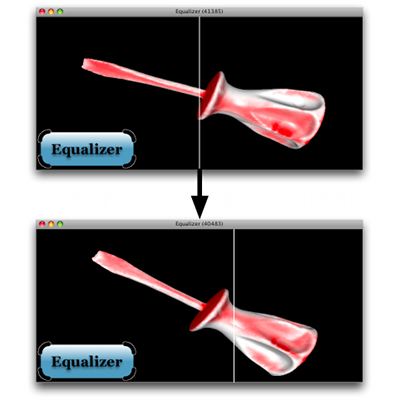
\includegraphics[width=\textwidth]{images/loadeq}
      \caption{\label{fig:loadeq}Load-Balancing}
  \end{subfigure}
  \begin{subfigure}[b]{0.24\textwidth}
    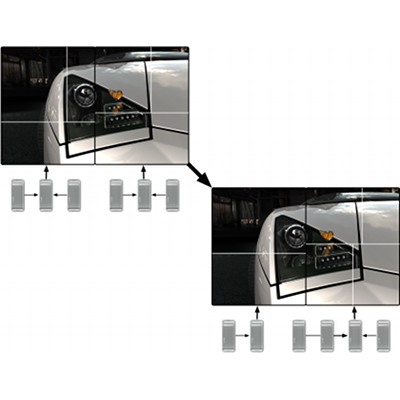
\includegraphics[width=\textwidth]{images/vieweq}
      \caption{\label{fig:vieweq}Cross-Segment Load-Balancing}
  \end{subfigure}
  \begin{subfigure}[b]{0.24\textwidth}
    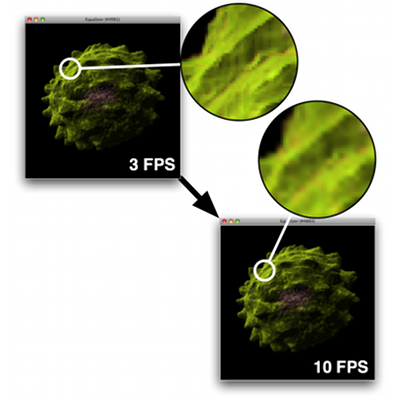
\includegraphics[width=\textwidth]{images/dfr}
      \caption{\label{fig:dfr}Dynamic Frame Resolution}
  \end{subfigure}
  \begin{subfigure}[b]{0.24\textwidth}
    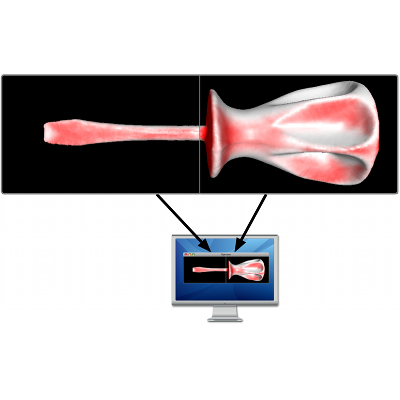
\includegraphics[width=\textwidth]{images/monitoreq}
      \caption{\label{fig:monitor}Monitoring}
  \end{subfigure}
  \caption{Runtime modifications}
  \label{fig:equalizers}
\end{figure*}

\subsubsection{Sort-First and Sort-Last Load Equalizer}

Sort-first (\fig{fig:loadeq}) and sort-last load balancing is the most obvious
optimization for these parallel rendering modes. Our load equalizer is fully
transparent for application developers, that is, it uses a reactive approach
based on past rendering times. This assumes a reasonable frame-to-frame
coherency. Our implementation stores a 2D or 1D grid of the load, mapping the
load of each channel. The load is stored in normalized 2D/1D coordinates using
$\frac{time}{area}$ as the load, the contributing source channels are organized
in a binary tree, and then the algorithm balances the two branches of each level
by equalizing the integral over the area on each side.

We have implemented various tunable parameters allowing application developers
to optimize the load balancing based on the characteristics of their rendering
algorithm:
\begin{compactdesc}
\item[Damping] reduces frame-to-frame oscillations. It is a normalized scalar
  defining how much of the computed delta from the previous position is
  applied. The equal load distribution within the region of interest assumed by
  the load equalizer is in reality not equal, causing the load balancing to
  overshoot.
\item[Resistance] eliminates small deltas in the load balancing step. This might
  help the application to cache some computations since the frustum does not
  change each frame.
\item[Boundaries] define the modulo factor in pixels onto which a load split may
  fall. Some rendering algorithms produce artefacts related to the OpenGL raster
  position, e.g., screen door transparency, which can be eliminated by aligning
  the boundary to the pixel repetition. Furthermore, some rendering algorithms
  are sensitive to cache alignments, which can again be exploited by chosing the
  corresponding boundary.
\end{compactdesc}

\subsubsection{Cross-Segment Load Balancing}

Cross-segment load balancing (\fig{fig:vieweq}) addresses the optimal resource
allocation of $n$ rendering resources to $m$ output channels (with $n\geq
m$). The view equalizer works in conjunction with load equalizer balancing the
individual output channels. It monitors the usage of shared source channels
(across outputs) and activates them to balance the rendering time of all
outputs. In \cite{EEP:11}, we provide a detailed description and evaluation of
our algorithm.

\subsubsection{Dynamic Frame Resolution}

The DFR equalizer (\fig{fig:dfr}) provides a functionality similar to dynamic
video resizing \cite{MBDM:97}, that is, it maintains a constant framerate by
adapting the rendering resolution of a fill-limited application. In Equalizer,
this works by rendering into a source channel (typically on a FBO) separate to
the destination channel, and then scaling the rendering during the transfer
(typically through an on-GPU texture) to the destination channel. The DFR
equalizer monitors the rendering performance and accordingly adapts the
resolution of the source channel and zoom factor for the source to destination
transfer. If the performance and source channel resolutions allows, this will
not only subsample, but also supersample the destination channel to reduce
aliasing artefacts.

\subsubsection{Frame Rate Equalizer}\label{sec:framerateEq}

The framerate equalizer smoothens the output frame rate of a destination
channel by instructing the corresponding window to delay its buffer swap to a
minimum time between swaps. This is regularly used for time-multiplexed
decompostions, where source channels tend to drift and finish their rendering
not evenly distributed over time. This equalizer is however fully independent of
DPlex compounds, and may be used to smoothen irregular application rendering
algorithms.

\subsubsection{Monitoring}

The monitor equalizer (\fig{fig:monitor}) allows to reuse the rendering on
another channel, typically for monitoring a larger setup on a control
workstation. Output frames on the display channels are connected to input frames
on a single monitoring channel. The monitor equalizer changes the scaling factor
and offset between the output and input, so that the monitor channel has the
same, but typically downscaled view, as the originating segments.

\subsection{Optimizations}

\subsubsection{Region of Interest}

The region of interest is the screen-space 2D bounding box enclosing the
geometry rendered by a single resource. We have extended the core parallel
rendering framework to use an application-provided ROI to optimize the load
equalizer as well as image compositing performance. The load equalizer uses the
ROI to refine its load grid to the regions containing data. The compositing code
uses the ROI to minimize image readback and network transmission. In
\cite{MEP:10} and \cite{EBAHMP:12}, we provide the details of the algorithm, and
show that using ROI can quadruple the rendering performance, in particular for
the costly compositing step in sort-last rendering.

\subsubsection{Asynchronous Compositing}

Asynchronous compositing pipelines rendering with compositing operations, by
executing the image readback, network transfer and image assembly from threads
running in parallel to the rendering threads. In \cite{EBAHMP:12}, we provide
the details of the implementation and experimental data showing an improvement
of the rendering performance of over 25\% for large node counts.

\subsubsection{Download and Compression Plugins}

Compression for the compositing step in parallel rendering is critical for
performance. This not only applies to the well-researched network transfer step,
but also for the transfer between GPU and CPU. Equalizer supports a variety of
compression algorithms, from very fast RLE encoding, JPEG compression to YUV
subsampling on the GPU. These algorithms are implemented as runtime-loaded
plugins, allowing easy extension and customization to application-specific
compression. In \cite{MEP:10}, we show this to be a critical step for
interactive performance at scale.

\subsubsection{Thread Synchronization Modes}\label{sec:threading}

Different applications have different degrees on how decoupled and thread-safe
the rendering code is from the application logic. For full decoupling all
mutable data has to have a copy in each render thread, which is not feasible in
large data scenarios. To easily customize the synchronization of all threads on
a single process, Equalizer implements three threading modes:  Full
synchronization, draw synchronization and asynchronous. Note that the execution
between nodes is always asynchronous, for up to \textsf{latency} frames.

In full synchronization, all threads always execute the same frame, that is, the
render threads are unlocked after \textsf{Node::frameStart}, and the node is
blocked for all render threads to finish the frame before executing
\textsf{Node::frameFinish}. This allows the render threads to read shared data
from all their operations, but provides the slowest performance.

In draw synchronization, the node thread and all render threads are synchronized
for all \textsf{frameDraw} operations, that is, \textsf{Node::frameFinish} is
executed after the last channel is done drawing. This allows the render threads
to read shared data during their draw operation, but not during
compositing. Since compositing is typically independent of the rendered data,
this is the default mode. This mode allows to overlap compositing with data
synchronization on multi-GPU machines.

In asynchronous execution, all threads run asynchronously. Render threads may
work on different frames at any given time. This mode is the fastest, and
requires the application to have one instance of each mutable object in each
render thread. It is required for using time-multiplex compounds in
multithreaded rendering.

%------------------------------------------------------------------------------
\section{Virtual Reality}
%------------------------------------------------------------------------------

Virtual Reality is an important field for parallel rendering. It does however
require special attention to support it as a first-class citizen in a generic
parallel rendering framework. Equalizer has been used in many virtual reality
installations, such as the Cave2 (\cite{FNTTL:13}), the high-resolution C6 CAVE
at the KAUST visualization laboratory and head-mounted displays
(\fig{FIG_teaser}). In the following we lay out the features needed support
these installations. All features presented were motivated by application use
cases and have been validated with their respective users.

\subsection{Head Tracking}

Head tracking is the minimal feature needed to support immersive
installations. Equalizer does support multiple, independent tracked views
through the observer abstraction introduced in \sref{sec:observer}. Built-in
VRPN support enables the direct, application-transparent configuration of a VRPN
tracker device. Alternatively, an application can provide a $4\times 4$ tracking
matrix defining the transformation from the canvas coordinate system to the
observer. Both CAVE-like tracking with fixed projection surfaces and HMD
tracking modes are implemented.

\subsection{Dynamic Focus Distance}

To our knowledge, all parallel rendering systems have the focal plane coincide
with the physical display surface. For better viewing comfort, we introduce a
new dynamic focus mode, where the application defines the distance of the focal
plane from the observer, based on the current view direction af the
user. Initial experiments show that this is particularly effective for objects
placed within the immersive space, that is, in front of all display segments.

\subsection{Asymmetric Eye Position}

Traditional head tracking computes the left and right eye positions by using a
configurable interocular distance and the tracking matrix. However, human heads
are not symmetric, and by measuring individual users a more precise frustum can
be computed. Equalizer supports this through the optional configuration (file or
programmatically) of individual 3D positions for the left and right eye.

\subsection{Model Unit}

This feature allows applications to specify a scaling factor between the model
and the real world, to allow exploration of macroscopic or microscopic worlds in
virtual reality. The unit is per view, allowing different scale factors within
the same configuration. It scales both the specified projection surface as well
as the eye position (and therefore separation) to achieve the necessary effect.

\subsection{Runtime Stereo Switch}

Applications can switch each view between mono and stereo rendering at runtime,
and can run both monoscopic and stereoscopic views concurrently
(\fig{FIG_teaser} (b)). While this is trivial for active stereo rendering, it
does potentially involve the start and stop of resources and processes for
passive stereo or stereo-dependent task decompositions, as described in
\sref{sec:reconfig}.

%------------------------------------------------------------------------------
\section{Usability}
%------------------------------------------------------------------------------

In this section we present features motivated by real-world application use
cases, i.e., new functionalities rather then performance improvements. We
motivate the use case, explain the architecture and integration into our
parallel rendering framework, and, where applicable, show the steps needed to
use this functionality in applications.

\subsection{Physical and Logical Visualization Setup}

Real-world visualization setups are often complex, and having an abstract
representation of the display system can simplify the configuration
process. Real-world applications often have the need to be aware of spatial
relationship of the display setup, for example to render 2D overlays or to
configure multiple views on a tiled display wall.

We addressed this need through a new configuration section interspersed between
the node/pipe/window/channel hardware resources and the compound trees
configurating the resource usage for parallel rendering.

A typical installation consists of one projection canvas, which is one
aggregated projection surface, e.g., a tiled display wall or a CAVE. Desktop
windows are considered a canvas. Each canvas is made of one or more segments,
which are the individual outputs connected to a display or projector. Segments
can be planar or non-planar to each other, and can overlap or have gaps between
each other. A segment is referencing a channel, which defines the output area of
this segment, e.g., on a DVI connector connected to a projector.

A canvas can define a frustum, which will create default, planar sub-frusta for
all of its segments. A segment can also define a frustum, which overrides the
canvas frustum, e.g., for non-planar setups such as CAVEs or curved
screens. These frusta describe a physically-correct display setup for a Virtual
Reality installation. \label{sec:swap} A canvas may have a software or hardware
swap barrier, which will synchronize the rendering of all contributing GPUs. The
software barrier executes a \textsf{glFinish} to ensure the GPU is ready to
swap, a Collage barrier (\sref{sec:barrier}) to synchronize all segments, the
swap buffers call followed by a \textsf{glFlush} to ensure timely execution of
the swap command. The hardware swap barrier is implemented using the
\textsf{WGL\_NV\_swap\_group} or \textsf{GLX\_NV\_swap\_group} extensions.

On each canvas, the application can display one or more views. A view is a view
on a model, in the sense used by the MVC pattern. The view class is used by
Equalizer applications to define view-specific data for rendering, e.g., a
scene, viewing mode or camera. The application process manages this data, and
the render clients receive it for rendering.

A layout groups one or more views which logically belong together. A layout is
applied to a canvas. The layout assignment can be changed at run-time by the
application. The intersection between views and segments defines which output
channels are available, and which frustum they should use for rendering. These
output channels are then used as destination channels in a compound. They are
automatically created during configuration.

A view may have a frustum description. The view's frustum overrides frusta
specified at the canvas or segment level. This is used for non-physically
correct rendering, e.g., to compare two models side-by-side on a tiled display
wall. If the view does not specify a frustum, the corresponding destination
channels will use the physically correct sub-frustum resulting from the
view/segment intersection.

\label{sec:observer}
An observer looks at one or more views. It is described by the observer position
in the world and its eye separation. Each observer will have its own stereo
mode, focus distance and frame loop (framerate). This allows to have untracked
views and multiple tracked views, e.g., two HMDs, in the same application.

\subsection{Runtime Reconfiguration}\label{sec:reconfig}

Switching a layout, as described above, or switching the stereo rendering mode,
may involve a different set of resources after the change, including the launch
and exit of render client processes. Equalizer solves this through a
reconfiguration step at the beginning of each rendering frame. Each resource
(channel, window, pipe, node) has an activation count, which is updated when the
layout or any other relevant rendering parameter is changed. When a resource is
found whose activation count does not match its current start/stopped state, the
resource is created or destroyed and \textsf{configInit} or \textsf{configExit}
are called accordingly. In the current implementation, a normal configuration
initialization or exit, as described in \cite{EMP:09}, uses the same code path
with all used resources transitioning to a running or stopped state,
accordingly. Since starting new resources typically requires object mapping and
associated data distribution, it is a costly operation. To improve performance
and robustness, Equalizer will flush the rendering pipeline whenever a runtime
reconfiguration is detected, before executing the change. This implementation
allows the late join or early exit, transparent to application developers.


\subsection{Automatic Configuration}

Automatic configuration implements the discovery of local and remote resources
as well as the creation of typical configurations using the discovered resources
at application launch time.

The discovery is implemented in a separate library, hwsd (HardWare Service
Discovery), which uses a plugin-based approach to discover GPUs for GLX, AGL or
WGL windowing systems, as well as network interfaces on Linux, Mac OS X and
Windows. Furthermore, it detects the presence of VirtualGL to allow optimal
configuration of remote visualization clusters. The resources can be discovered
on the local workstation, and through the help of a simple daemon using the
zeroconf protocol, on a set of remote nodes within a visualization cluster. A
session identifier may be used to support multiple users on a single cluster.

The Equalizer server uses the hwsd library to discover local and remote
resources when an hwsd session name instead of a \textsf{.eqc} configuration
file is provided. A set of standard decomposition modes is configured, which can
be selected through activating the corresponding layout.

This versatile mechanism allows non-experts to configure asnd profit from
multi-GPU workstations and visualization clusters, as well as to provide system
administrators with the tools to implement easy to use integration with cluster
schedulers. This feature is transparent to Equalizer application developers.

\subsection{Qt Windowing}

Qt is a popular window system with many application developers. Unfortunately,
it imposes a different threading model for window creation and event handling
compared to Equalizer. In Equalizer, each GPU rendering thread is independently
responsible for creating its windows, receiving the events and eventually
dispatching them to the application process main thread. This design is
motivated by the natural threading model of X11 and WGL, and allows simple
sequential semantics between OpenGL rendering and event handling. In contrast,
Qt requires all windows and QOpenGLContext to be created from the Qt main
thread. An existing Qt window or context may be moved to a different thread, and
events are signalled from the main thread.

Challenges in threading model, architecture

\subsection{Tide Integration}

Tide (Tiled interactive display environment) is an improved version of
DisplayCluster~\cite{DC}, providing touch-based, multi-window user interface for
high-resolution tiled display walls. Remote applications receive input events
and send pixel streams using the Deflect client library. Equalizer includes full
support, enabling application-transparent integration with Tide. When a Tide
server is configured, all output channels of a view stream in parallel to one
window on the wall. In \cite{deflect} we have shown interactive framerates for
an 24 megapixel resolution over a WAN link. Events received are translated into
Equalizer events and injected into the normal event flow, allowing seamless
application integration.

\subsection{Sequel}\label{sec:sequel}

Sequal is a simplification layer for Equalizer. It is based on the realization
that while fully expressive, the verbatim abstraction layer of nodes, pipes,
windows and channels in Equalizer requires significant learning to fully
understand and exploit. In reality, a higher abstraction of \textsf{Application}
and \textsf{Renderer} is sufficient for most use cases. In Sequel, the
application class drives the configuration, and one renderer instance is created
for each (pipe) render thread. They also provide the natural place to store and
distribute data. Last, but not least, \textsf{ViewData} provides a convenient
way to manage multiple views by storing the camera, model or any other
view-specific information.

%------------------------------------------------------------------------------
\section{The Collage Network Library}
%------------------------------------------------------------------------------

An important part of writing a parallel rendering application is the
communication layer between the individual processes. Equalizer relies on the
Collage network library for its internal operation. Collage furthermore provides
powerful abstractions for writing Equalizer applications, which are introduced
in this section.

\subsection{Architecture}

Collage provides networking functionality of different abstraction layers,
gradually providing higher level functionality for the programmer. The main
primitives in Collage are:

\begin{compactdesc}
\item[Connection] A stream-oriented point-to-point communication
  line. The connections
  transmit raw data reliably between two endpoints for unicast connections, and
  between a set of endpoints for multicast connections. For unicast,
  process-local pipes, TCP and Infiniband RDMA are implemented. For multicast,
  a reliable, UDP-based protocol is discussed in \sref{sec:RSP}.
\item[DataI/OStream] Abstracts the input and output of C++ data types from or to
  a set of connections by implementing output stream operators. Uses buffering
  to aggregate data for network transmission. Performs endian swapping during
  input if the endianness differs between the originating and local node.
\item[Node and LocalNode] The abstraction of a process in the cluster. Nodes
  communicate with each other using connections. A LocalNode listens on various
  connections and processes requests for a given process. Received data is
  wrapped in ICommands and dispatched to command handler methods. A Node is a
  proxy for a remote LocalNode. The Equalizer Client object is a LocalNode.
\item[Object] Provides object-oriented, versioned data distribution of C++
  objects between nodes. Objects are registered or mapped on a Local\-Node.
\end{compactdesc}

\begin{figure}[ht]\center
  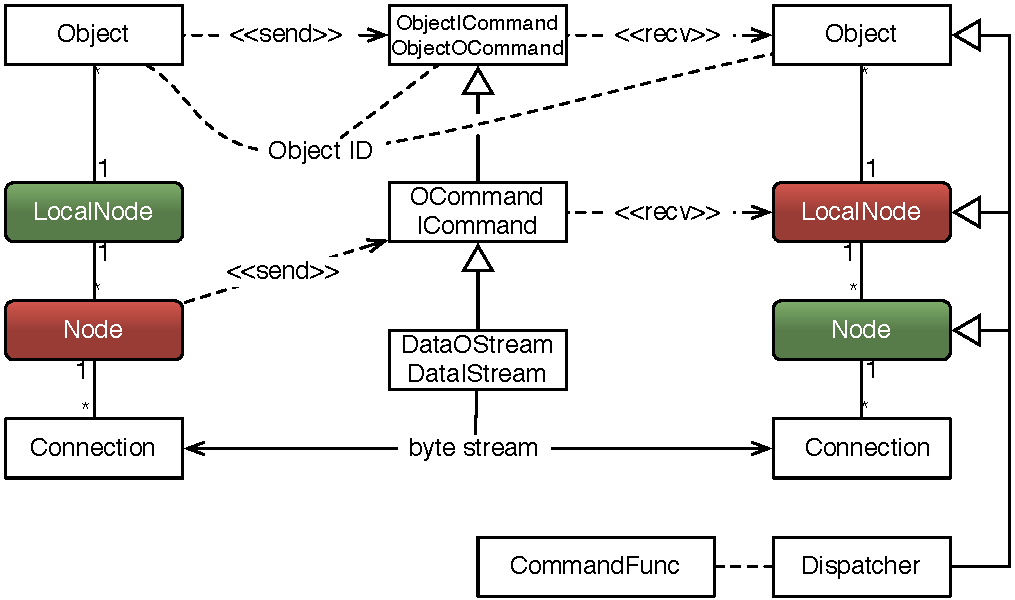
\includegraphics[width=\columnwidth]{EqDocs/Developer/ProgrammingGuide/images/netObject}
  \caption{\label{fNetObject}Communication between two Collage Objects}
\end{figure}
\fig{fNetObject} illustrates this architecture.

\subsection{Infiniband RDMA}

needed? reverse-engr impl

\subsection{Reliable Stream Protocol}\label{sec:RSP}

RSP is an implementation of a reliable multicast protocol over unreliable UDP
transport. RSP behaves similarly to TCP, it provides full reliability and
ordering of the data, and slow receivers will eventually throttle the
sender. This behaviour is needed to guarantee delivery of data in all
situations. Pragmatic generic multicast (PGM~\cite{pgm}) provides full ordering,
but slow clients will disconnect from the multicast session instead of
throttling the send rate.

RSP combines various established algorithms~\cite{adamson2004negative,
  Gau:2002:MFC:506824.506832} for multicast in an open source implementation
capable of delivering wire speed transmission rates on high-speed LAN
interfaces. In the following we will outline the RSP protocol and implementation
and motivate the design decisions. Any defaults given below are for Linux or OS
X, the Windows UDP stack requires different default values which can be found in
the implementation.

Our RSP implementation uses a separate protocol thread for each RSP connection,
which handles all reads and writes on the multicast group. This thread
implements the protocol handling and communicates with the application threads
through thread-safe queues, as shown in \fig{fRSPProto}. These queues contain
datagrams, which are prefixed by a type-specific header. Each connection has a
configurable number of buffers, (1024 by default) of a configurable MTU (1470
bytes default) which are either free for use or in-use for reading or writing.

%%     1,     // RSP_ERROR_DOWNSCALE
%%     5,     // RSP_ERROR_UPSCALE
%%     20,    // RSP_ERROR_MAXSCALE
%%     3,     // RSP_MIN_SENDRATE_SHIFT

%%     17,    // RSP_ACK_FREQUENCY


\begin{figure}[ht]\center
  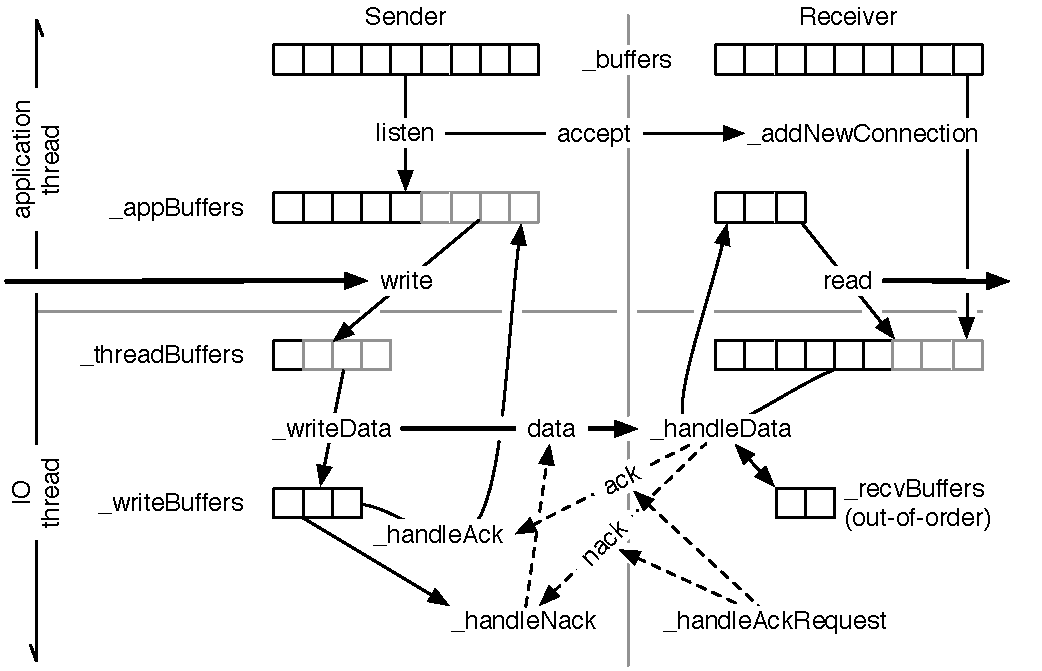
\includegraphics[width=\columnwidth]{images/rspPackets}
  \caption{\label{fRSPProto}Reliable Stream Protocol}
\end{figure}

A client opens a listening multicast RSP connection. Similar to TCP, this
listener will create one connected RSP connection for each remote member in the
multicast group, that is, on each node $n$ RSP connection instances exist, $1$
for the local listener and $n-1$ for all other nodes. A multicast group
therefore looks like a fully connected set of TCP connections between $n$ nodes
for the user.

Each member of a multicast group has a group-unique 16 bit identifier, which is
randomly selected, announced to the group, and if no collisions are notified by
any other member, confirmed for this connection. This mechanism allows
addressing of connections with a low protocol overhead. The datagrams used in
this exchange contain no payload, and they contain two bytes type (HELLO,
HELLO\_REPLAY, HELLO\_DENY, HELLO\_CONFIRM), two bytes protocol version and two
bytes connection identifier.

The \textsf{\_appBuffers} queue, which is blocking, contains received UDP
datagrams on incoming connections, or empty buffers for writing on outgoing
connections. The \textsf{\_threadBuffers} queue is lock-free and used by the
protocol thread to store empty buffers on incoming connections, and pre-packaged
UDP datagrams on outgoing connections. The application thread pushes buffers
into this queue, consumed by the protocol thread. A datagram is up to 64
kilobytes (UDP limit, configurable) and contains a header (two bytes type, two
bytes size, two bytes source identifier, two bytes sequence number) and its
payload. The sequence number is used for positive (ack) and negative (nack)
acknowledgments and reordering of packets.

The \textsf{\_writeBuffers std::deque} is only used by the protocol
thread. It contains already sent, but not yet acknowledged datagrams. Its
datagrams are resent upon reception of a nack or recycled into
\textsf{\_appBuffers} when acknowledged by all receivers. Similarly, the
\textsf{\_recvBuffers std::deque} contains received out-of-order packets already
received by an incoming connection. Upon each reception it is checked, and
in-order datagrams are placed into \textsf{\_appBuffers} for consumption by the
application thread.

Handling a smooth packet flow is critical for performance. RSP actively flow
control to advance the stream. Each incoming connection actively acknowledges
every $n$ (17 by default) packets fully received. The incoming connections shift
this acknowledgment by their connection identifier to avoid bursts of acks. Any
missed datagram is actively nack'ed as soon as it is detected. Write connections
continuously retransmit packets from nack datagrams, and advance their
\textsf{\_writeBuffers} upon reception of acks from all readers. Furthermore,
the writer will explicitly request an ack or nack when it runs out of empty
buffers or finishes its write queue.

Congestion control is necessary to optimize bandwidth usage. While TCP uses the
well-known AIMD (additive increase, multiplicative decrease) algorithm, we have
chosen a more aggressive congestion control algorithm of additive increase and
decrease. This has proven experimentally to be more optimal: UDP is often
rate-limited by switches, that is, packets are discarded regularly and not
exceptionally. Only slowly backing of the current send rate helps to stay close
to this limit. Furthermore, our RSP traffic is limited to the local subnet,
making cooparation between multiple data stream less of an issue. Send rate
limiting uses a bucket algorithm, where over time the bucket fills with send
credits, from which sends are substracted. If there are no available credits,
the sender sleeps until sufficient credits are available.

\subsection{Distributed, Versioned Objects}

Adapting an existing application for parallel rendering requires the
synchronization of application data across the processes in the parallel
rendering setup. Existing parallel rendering frameworks address this often
poorly, at best they rely on MPI to distribute data. Real-world, interactive
visualization applications are typically written in C++ and have complex data
models and class hierarchies to represent their application state. As outlined
in \cite{EMP:09}, the parallel rendering code in an Equalizer application only
needs access to the data needed for rendering, as all application logic is
centralized in the application main thread. We have encountered two main
approaches to address this distribution: Using a shared filesystem for static
data, or using data distribution for static and dynamic data.

Distributed objects are not required to build Equalizer applications. While most
developers choose to use this abstraction for convenience, we have seen
applications using other means for data distribution, e.g., MPI.

\subsubsection{Programming Interface}

Distributed objects in Collage provide powerful, object-oriented data
distribution for C++ objects. They facilitate the implementation of data
distribution in a cluster environment. Distributed objects are created by
subclassing from \textsf{co::Serializable} or \textsf{co::Object}. The
application programmer implements serialization and deserialization of the
distributed data. Distributed objects can be static (immutable) or
dynamic. Objects have a universally unique identifier (UUID) to address them
cluster-wide. A master-slave model is used to establish mapping and data
synchronization across processes. Typically, the application main loop registers
a master instance and communicates the UUID to the render clients, which map
their instance to the given identifier. The following object types are
available:

\begin{compactdesc}
\item[Static] The object is not versioned nor buffered. The instance data is
  serialized whenever a new slave instance is mapped. No additional data is
  stored.
\item[Instance] The object is versioned and buffered. The instance and delta
  data are identical, that is, only instance data is serialized. Previous
  instance data is saved to be able to map old versions.
\item[Delta] The object is versioned and buffered. The delta data is typically
  smaller than the instance data. The delta data is transmitted to slave
  instances for synchronization. Previous instance and delta data is saved to be
  able to map and sync old versions.
\item[Unbuffered] The object is versioned and unbuffered. No data is stored, and
  no previous versions can be mapped. No old versions can be mapped and no
  additional data is stored.
\end{compactdesc}

All distributed objects have to implement \textsf{getInstanceData} and
\textsf{applyInstanceData} to serialize and deserialize the object's distributed
data. These methods provide an output or input stream as a parameter, which
abstracts the data transmission and can be used like a \textsf{std::stream}.
The data streams implement efficient buffering and compression, and
automatically select the best connection for data transport. Custom data type
serializers can be implemented by providing the appropriate serialization
functions. No pointers should be directly transmitted through the data
streams. For pointers, the corresponding object is typically a distributed
object as well, and its identifier and potentially version is transmitted in
place of the memory address.

Dynamic objects are versioned, and have to override \textsf{getChangeType} to
indicate how they want to have changes to be handled. Upon \textsf{commit} the
delta data from the previous version is sent, if available using multicast, to
all mapped slave instances. The data is queued on the remote node, and is
applied when the application calls \textsf{sync} to synchronize the object to a
new version. The \textsf{sync} method might block if a version has not yet been
committed or is still in transmission. All versioned objects the following
characteristics:

\begin{compactitem}
\item The master instance of the object generates new versions for all
  slaves. These versions are continuous. It is possible to commit on slave
  instances, but special care has to be taken to handle possible
  conflicts.
\item Slave instance versions can only be advanced, that is, \textsf{sync(
  version )} with a version smaller than the current version will fail.
\item Newly mapped slave instances are mapped to the oldest available
  version by default, or to the version specified when calling
  \textsf{mapObject}.
\end{compactitem}

Besides the instance data serialization methods used to map an object, delta and
unbuffered objects may implement \textsf{pack} and \textsf{unpack} to serialize
or deserialize the changes since the last version.

\label{sec:Serializable}The Collage Serializable implements one convenient usage
pattern for object data distribution. The \textsf{co::Serializable} data
distribution is based on the concept of dirty bits, allowing inheritance with
data distribution. Dirty bits form a 64-bit mask which marks the parts of the
object to be distributed during the next commit. For serialization, the
application developer implements \textsf{serialize} or \textsf{deserialize},
which are called with the bit mask specifying which data has to be transmitted
or received. During a commit or sync, the current dirty bits are given, whereas
during object mapping all dirty bits are passed to the serialization methods.

Blocking commits allow to limit the number of outstanding, queued versions on
the slave nodes. A token-based protocol will block the commit on the master
instance if to many unsynchronized versions exist.

\subsubsection{Optimizations}

The API presented in the previous section provides sufficient abstraction to
implement various optimizations for faster mapping and synchronization of data:
compression, chunking, caching, preloading and multicast. The results section
evaluates these optimizations.

The most obvious one is compression. Recently, many new compression algorithms
have been developed which exploit modern CPU architectures and deliver
compression rates well above one gigabyte per second. Collage uses the Pression
library~\cite{pression}, which provides an unified interface for a number of
compression libraries, such as FastLZ~\cite{jesperfast}, Snappy~\cite{snappy}
and ZStandard~\cite{zstd}. It also contains a custom, virtually zero-cost RLE
compressor. Pression also parallelizes the compression and decompression using
data decomposition.

The data streaming interface also implements chunking, which aims to pipeline
the serialization code with the network transmission. After a configurable
number of bytes has been serialized to the internal buffer, it is transmitted
and serialization continues. This is used both for the initial mapping data and
for commit data.

Caching retains instance data of objects in a cache, and reuses this data to
accelarate mapping of objects. The instance cache is either filled by "snooping"
on multicast transmissions or by an explicit preloading when the master objects
are registered. The preloading ("send on register") sends instance data of
recently registered master objects while the correspinding node is idle to all
connected nodes. These nodes simply enter the received data to their
cache. Preloading uses multicast when available.

Due to the master-slave model of data distribution, multicast can be used to
optimize the transmission time of data. If the contributing nodes share a
multicast session, and more than one slave instance is mapped, Collage
automatically uses the multicast connection to send the new version
information.

\subsection{Barriers, Queues and Object Maps}\label{sec:barrier}

Collage implements a few generic distributed objects which are used by Equalizer
and applicatons. A barrier is a distributed barrier primitive used for software
swap barriers in Equalizer (\sref{sec:swap}). Its implementation follows a
simple master-slave approach, which has shown to by sufficient for this use
case. Queues are single producer, multiple consumer FIFOs. To hide network
latencies, the consumers use prefetching of queue items into a local queue. They
are used for tile and chunk compounds (\sref{sec:tile}).

The object map facilitates distribution and synchronization of a collection of
distributed objects. Master versions can be registered on a central node, e.g.,
the application node in Equalizer. Consumers, e.g., Equalizer render clients,
can selectively map the objects they are interested in. Committing the object
map will commit all registered objects and sync their new version to the
slaves. Syncing the map on the slaves will synchronize all mapped instances to
the new version recorded in the object map. This effective design allows data
distribution with minimal application logic. It is used by Sequel
(\sref{sec:sequel}) and other Collage applications.

%----------------------------------------------------------------------
\section{Applications}
%----------------------------------------------------------------------

In this section, we present some major applications built using Equalizer, and
show how they interact with the framework to solve complex parallel rendering
problems.

\subsection{Livre}

Livre (Large-scale Interactive Volume Rendering Engine) is an out-of-core
parallel 4D volume renderer. It supports sort-first decomposition, both for
scalability as well as for driving large-scale tiled display walls. The
out-of-core loading of data relies on a shared file system, only the high-level
state, e.g., camera position and rendering settings, are shared through Collage
objects.

\subsection{RTT Deltagen}

RTT Deltagen (now Dassault 3D Excite) is a commercial application for
interactive, high quality rendering of CAD data. The RTT Scale module,
delivering multi-GPU and distributed execution, is based on Equalizer and
Collage, and has driven many of the aforementioned features.

RTT Scale uses a master-slave execution mode, were a single running Deltagen
instance can go into "Scale mode" at any time by launching an Equalizer
configuration. Consequently, the whole internal representation needed for
rendering is based on a Collage-based data distribution. The rendering clients
are separate, smaller applications which will map their scenes during
startup. At runtime, any change performed in the main application is committed
as a delta at the beginning of the next frame, following a design pattern
similar to the Collage \textsf{Serializable}
(\sref{sec:Serializable}). Multicast (\sref{sec:RSP}) is used to keep data
distribution times during session launch reasonable for larger cluster sizes
(tens to hundreds of nodes).

RTT Scale is used for a wide variety of use cases. In virtual reality, the
application is used for virtual prototyping and design reviews in front of
high-resolution display walls or in a CAVE and for virtual prototyping of
human-machine interactions in a CAVE or using HMDs. For scalability, sort-first
and tile compounds are used to achieve fast, high-quality rendering, primarily
for interactive raytracing, both based on CPUs and GPUs. For CPU-based
raytracing, often Linux-based rendering clients are used with a Windows-based
application node.

\subsection{RTNeuron}
\cite{HBBES:13}

\subsection{Raster}

\subsection{Bino}

\subsection{Omegalib}

%----------------------------------------------------------------------
\section{Experimental Results}\label{sec:results}
%----------------------------------------------------------------------

hardware description

\subsection{Decomposition Modes}

Two graphs: Time to render a 4k, 256-step MSAA image of largest ply model and
Livre using 1..16 nodes with all modes (2D, 2D LB, DB, DPlex (over AA steps),
tiles, chunks, pixel, subpixel) (+DFR for Livre)

\subsection{Object Distribution}

To benchmark the data distribution we used two datasets: The david statue at 2mm
resolution (\fig{fDavid2mm}) and 3D volumes of a spike frequencies of an
electrical simulation of three million neurons (\fig{fVolumes}).

\begin{figure}[ht]\center
  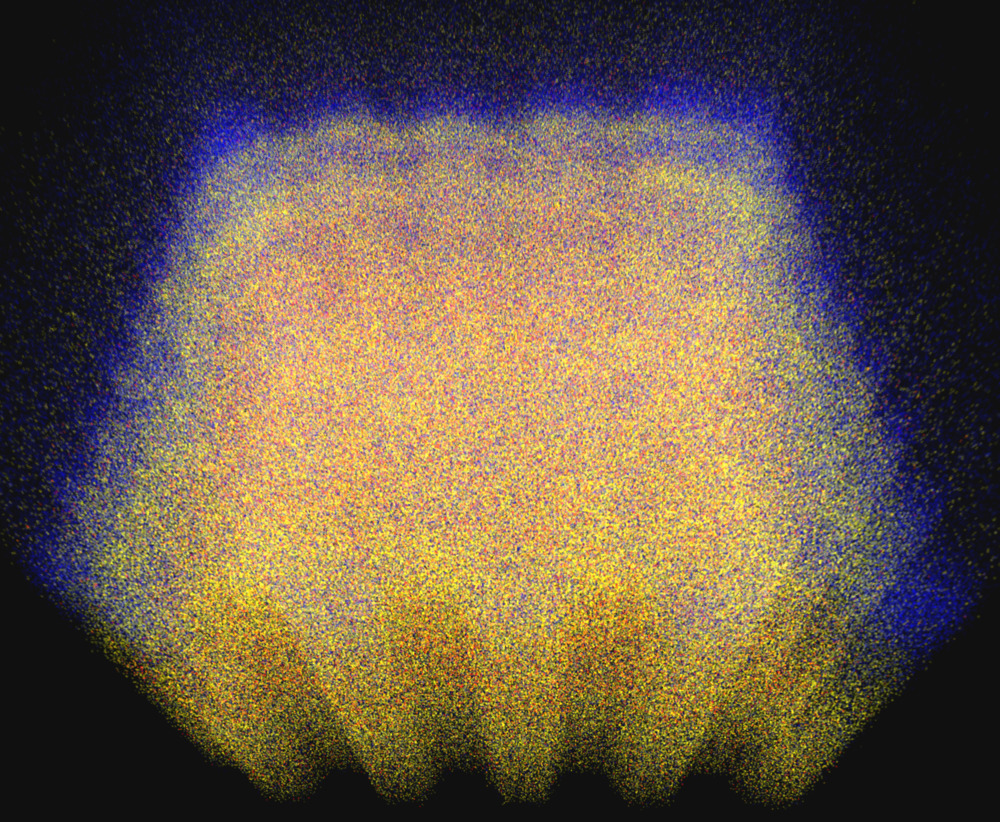
\includegraphics[width=.49\columnwidth]{images/spikes512}\hfil
  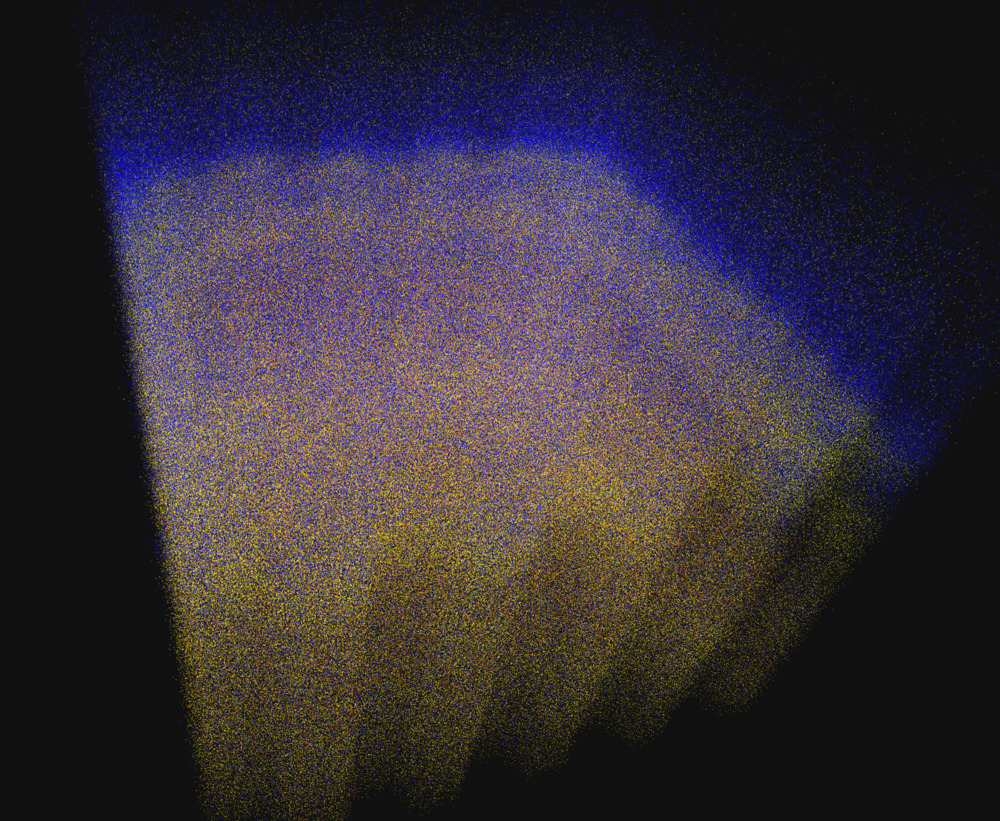
\includegraphics[width=.49\columnwidth]{images/spikes1280}
  \caption{\label{fVolumes}Spike frequencies of a three million neuron
    electrical simulation at 437x240x512 (51MB, left) and 1092x600x1280 (800MB,
    right) resolution}
\end{figure}

The spike frequency volumes aggregate the number of spikes which happened within
a given voxel over a given time. The absolute spike count is renormalized to an
unsigned byte value (0..255) during creation. Higher densities in the volume
represent higher spiking activity in the voxel. Consequently, the volume is more
sparsely populated and has a more even distribution of values at higher
resolution.

\subsubsection{Data Compression Engines}

A critical piece for data distribution performance are the characteristics of
the data compression algorithms. This microbenchmark compresses a set of binary
files to precalculate the speed and compression ratio of the various
engines. \fig{fCompressor} shows the compression and decompression speed in
gigabyte per second as well as the size of the compressed data. The different
ZSTD$x$ engines use the ZStandard compression library at level $x$.

\begin{figure}[ht]\center
  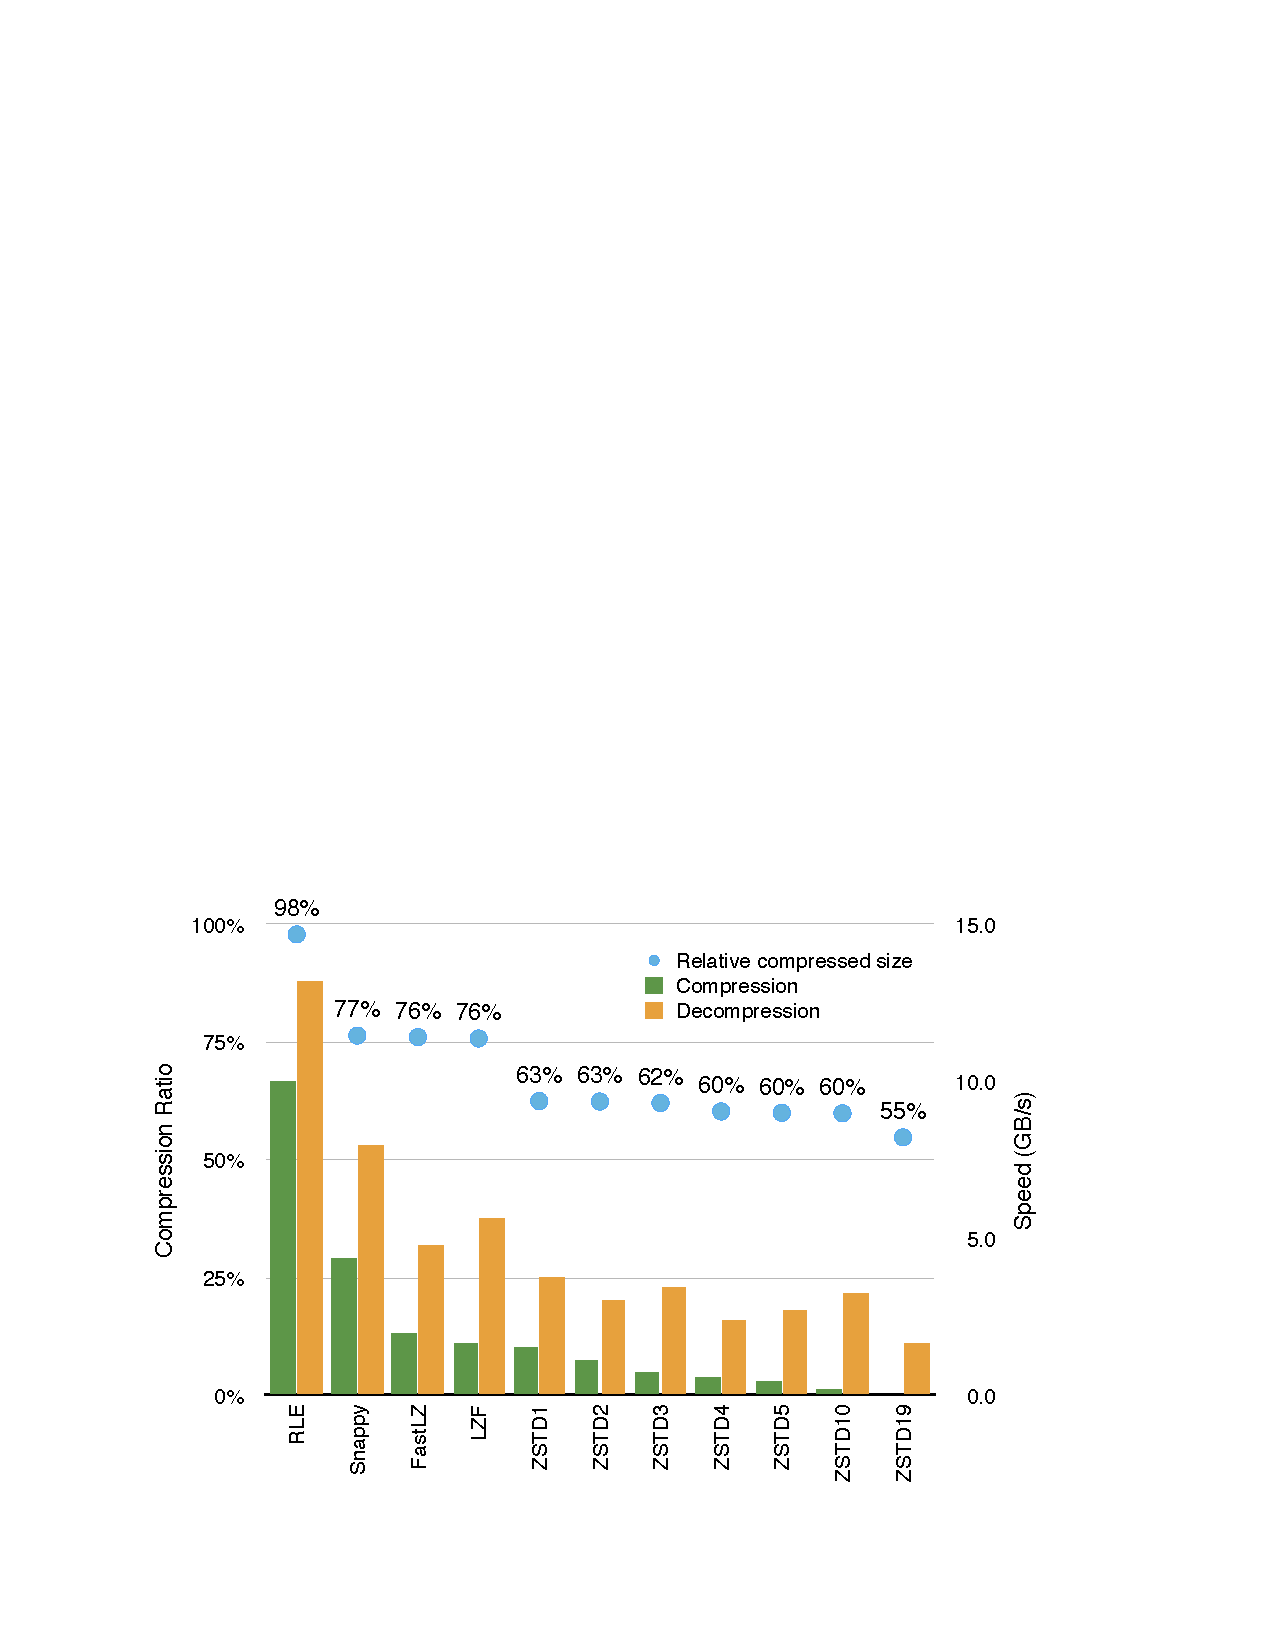
\includegraphics[width=\columnwidth]{images/compressor}
  \caption{\label{fCompressor}Data Compression for Generic Binary Data}
\end{figure}

RLE compression has a very low overhead, but does not compress the data will
since it only removes "blank space" in the data. The Snappy compression, used as
default in Collage, achieves the same compression ratio as the LZ variants at a
much higher speed. The ZStandard compressor has roughly the same speed as the LZ
variants at the lowest compression level, but provides significantly better
compression. At higher compression levels it can improve the compression ratio
slightly, but at a high cost for the compression speed.

The compression ratio for the models used in the following benchmark deviate
from this averaged distribution. \fig{fCompressorDetail} shows the compression
ratios for the triangle and volume data.

\begin{figure*}[ht]\center
  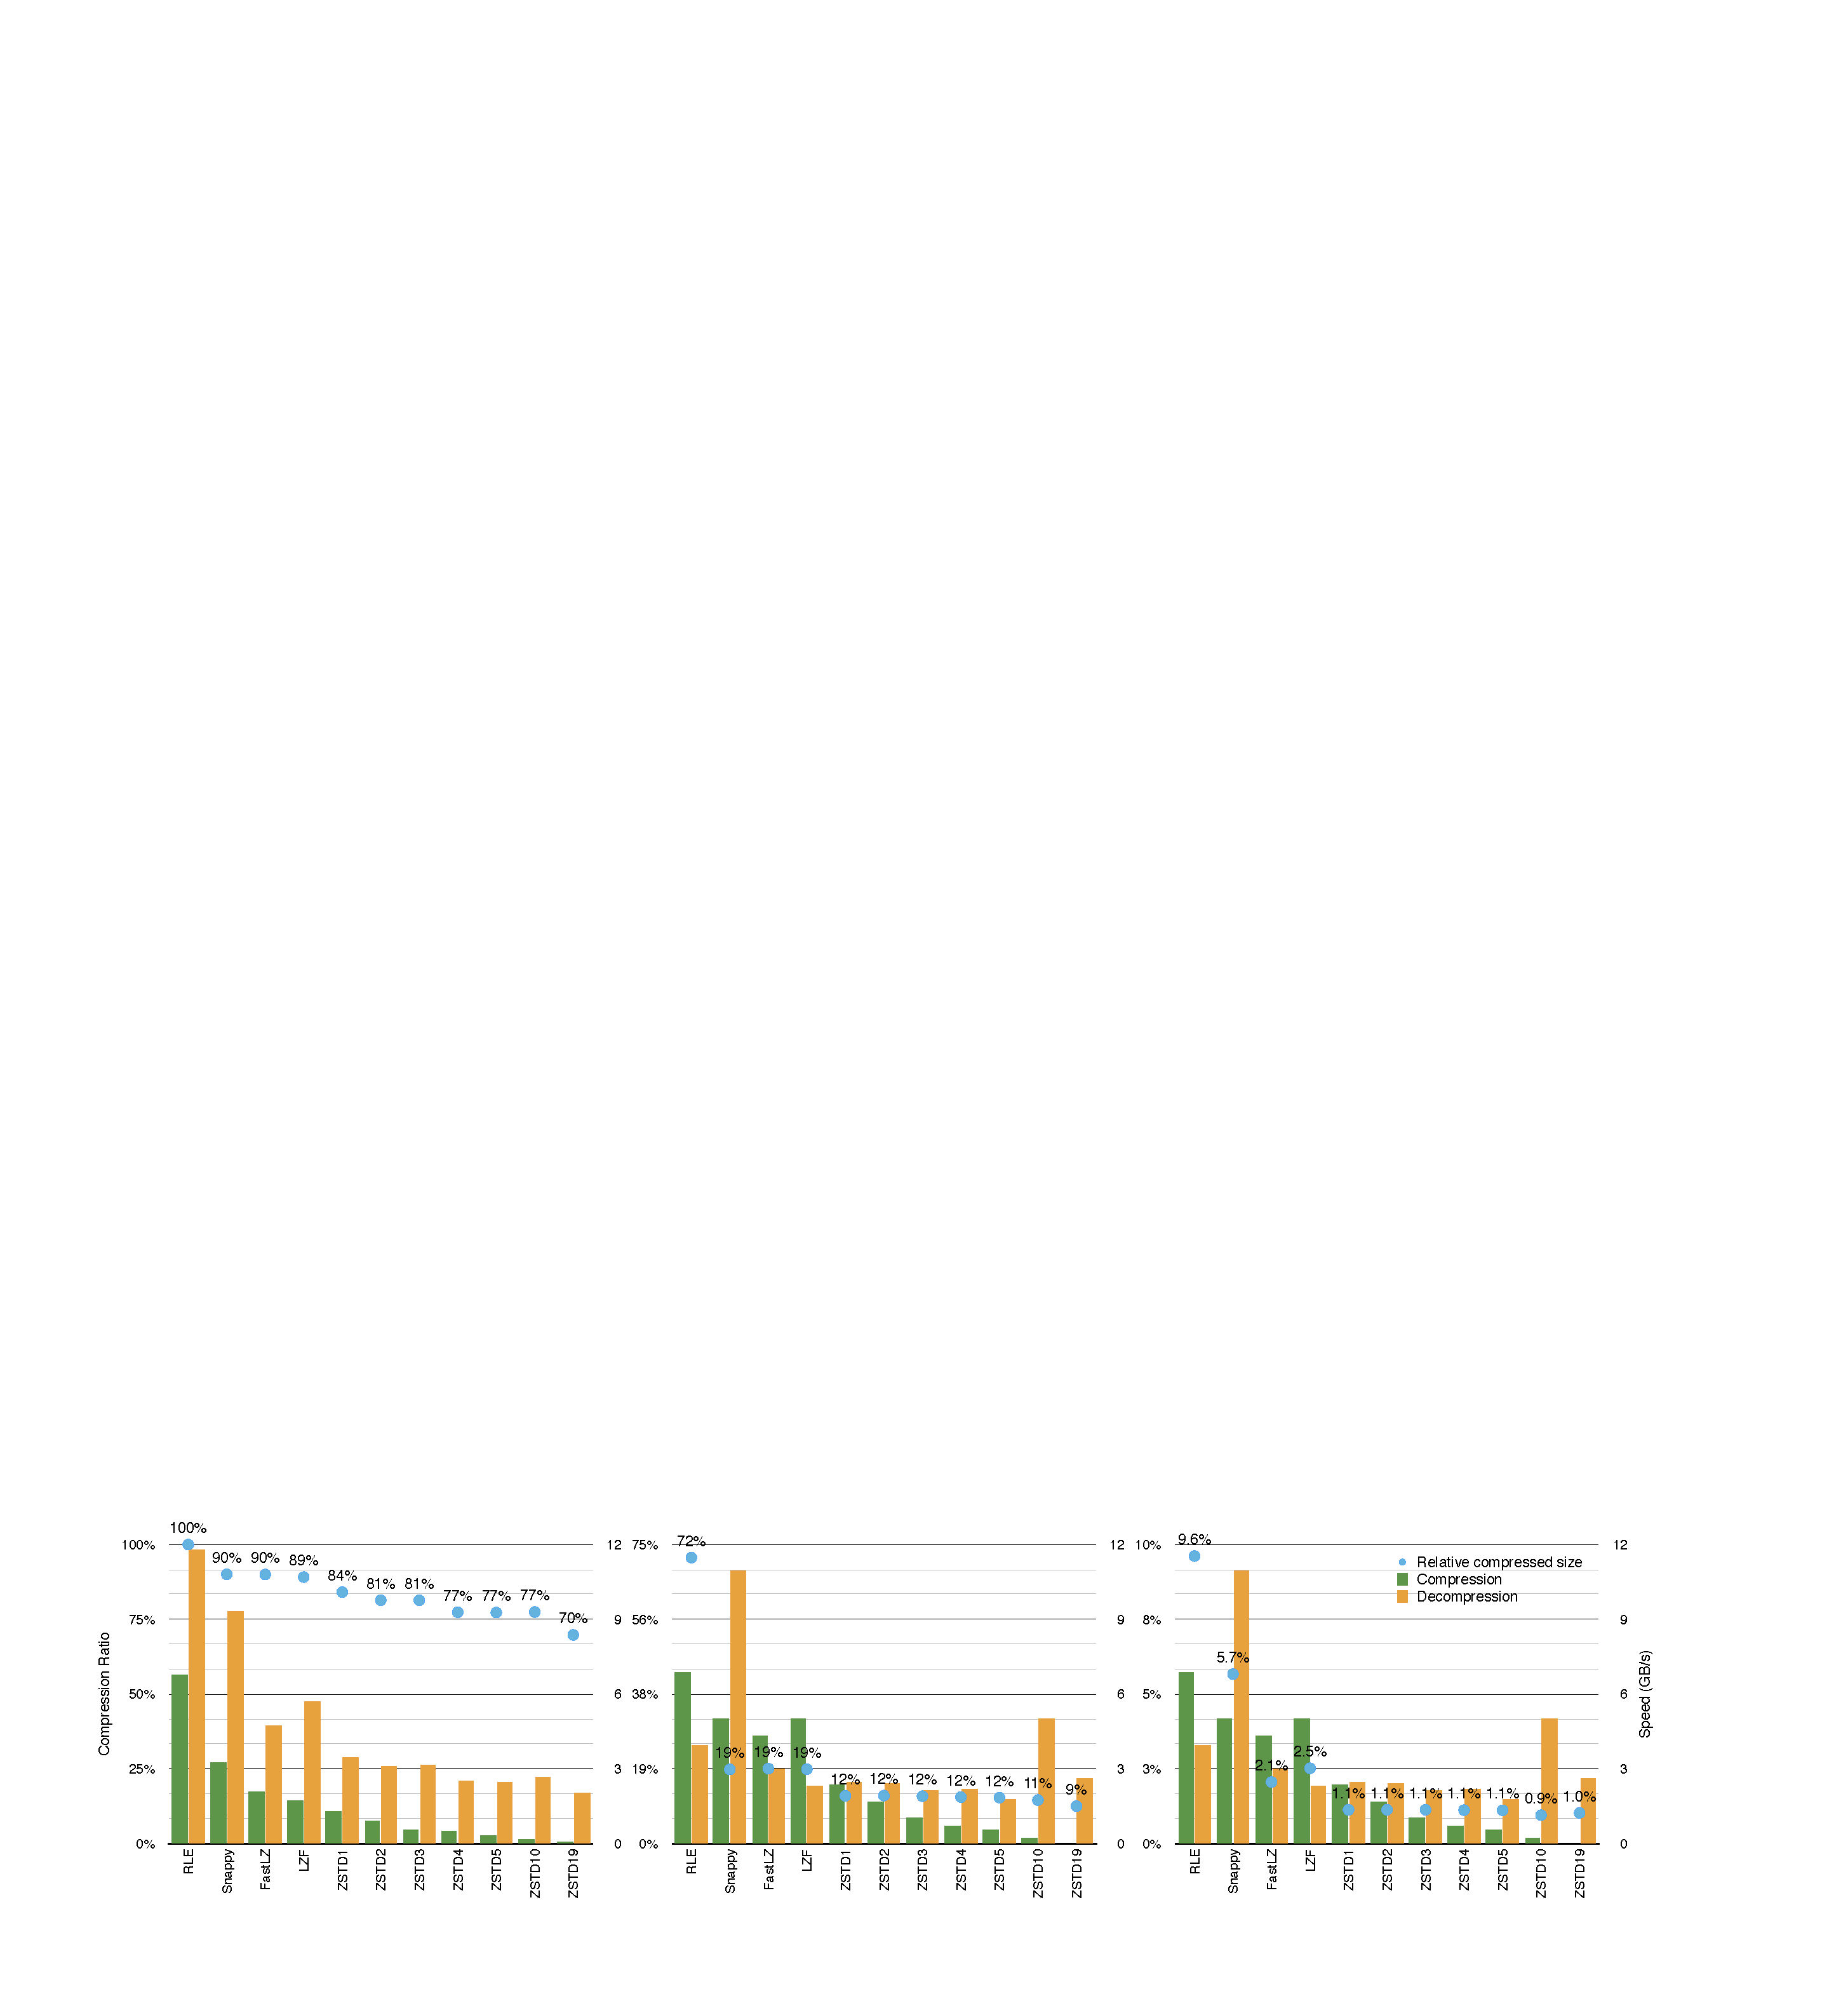
\includegraphics[width=\textwidth]{images/compressorDetail}
  \caption{\label{fCompressorDetail}Data Compression for ply data (left, David
    statue 2mm) and raw volume data shown in \fig{fVolumes} (middle and right)}
\end{figure*}

The ply data is little compressible, the default compressor achieves a 10\%
reduction. This is due to a high entropy in the data and the dominant use of
floating point representations. Overall the profile is similar to the generic
benchmark, at a smaller compression rate.

The volume data on the other hand is sparsely populated and using integer (byte)
representation, which is easier to compress. The naive RLE implementation
already achieves a good compression, showing that the smaller volume contains at
most 28\% empty space and the bigger volume at most 90\%. Snappy and ZStandard
can reduce the data much further, reducing the data to a few megabytes.


\subsubsection{Model Distribution and Update}
Distribute large ply and raw model to 1..16 nodes using TCP, IB and RSP

Distribute a video texture (per frame)

%----------------------------------------------------------------------
\section{Discussion and Conclusion}
%----------------------------------------------------------------------
\label{sec:conclusions}


%----------------------------------------------------------------------
\appendices
% use section* for acknowledgment
\ifCLASSOPTIONcompsoc
  % The Computer Society usually uses the plural form
  \section*{Acknowledgments}
\else
  % regular IEEE prefers the singular form
  \section*{Acknowledgment}
\fi
%----------------------------------------------------------------------
We would like to thank and acknowledge the following institutions and projects
for providing the 3D geometry and volume test data sets: the Digital
Michelangelo Project, Stanford 3D Scanning Repository, Cyberware Inc.,
volvis.org and the Visual Human Project.  This work was partially supported by
the Swiss National Science Foundation Grant 200021-116329/1.

We would also like to thank all supporters and contributors of Equalizer, most
notably RTT, the Blue Brain Project, the University of Siegen, EVL, Dardo, TBD.

% trigger a \newpage just before the given reference
% number - used to balance the columns on the last page
% adjust value as needed - may need to be readjusted if
% the document is modified later
%\IEEEtriggeratref{8}
% The "triggered" command can be changed if desired:
%\IEEEtriggercmd{\enlargethispage{-5in}}

% biography section
%
% If you have an EPS/PDF photo (graphicx package needed) extra braces are
% needed around the contents of the optional argument to biography to prevent
% the LaTeX parser from getting confused when it sees the complicated
% \includegraphics command within an optional argument. (You could create
% your own custom macro containing the \includegraphics command to make things
% simpler here.)
%\begin{IEEEbiography}[{\includegraphics[width=1in,height=1.25in,clip,keepaspectratio]{mshell}}]{Michael Shell}
% or if you just want to reserve a space for a photo:

\begin{IEEEbiography}{Michael Shell}
Biography text here.
\end{IEEEbiography}

% if you will not have a photo at all:
\begin{IEEEbiographynophoto}{John Doe}
Biography text here.
\end{IEEEbiographynophoto}

% insert where needed to balance the two columns on the last page with
% biographies
%\newpage

\begin{IEEEbiographynophoto}{Jane Doe}
Biography text here.
\end{IEEEbiographynophoto}

\bibliographystyle{abbrv}
\bibliography{references}

% that's all folks
\end{document}
